\section {Sulfur Dioxide Bonding Coordinations}

To further assess the effect of temperature on \suldiox~behavior we turn to analysis of the bonds formed between \suldiox~and the water surface. The bonding coordinations were determined for the \suldiox~based on the bondlength criteria noted in the introduction. Bonds formed between \suldiox-sulfur and \wat-oxygen are labeled 'S' coordinated, and bonds formed between \suldiox-oxygen and \wat-hydrogen are labeled 'O' coordinated. For each bond an additional letter label is appended to the coordination. For example, an 'SOO' coordinated \suldiox~forms three bonds to waters: two bonds are formed through the \suldiox-oxygens, and one through the \suldiox~sulfur. This naming scheme is taken from a similar convention used for describing water bonding interactions, but applied now to the \suldiox~molecule.\cite{Buch2005} 

Figure \ref{fig:so2-bonding-coordinations} shows the distribution of bonding coordinations throughout the set of simulated trajectories for both the cold and hot temperatures. The two most common coordination types are the S and SO, followed by a completely unbound \suldiox~molecule. Bonding is primarily found through the \suldiox-sulfur atom, with higher coordinationsThe distribution shows that the \suldiox~mostly forms one or two bonding interactions with the waters. The bonding of the \suldiox~at both low and high temperatures follows similar trends, however the higher temperature shifts the distribution of coordinations slightly to forming more bonds than the cold temperature \suldiox. Figure \ref{fig:coordination-breakdown} breaks down the coordination distribution to show more details of the \suldiox~interactions.

The total number of bonds formed to the \suldiox~are shown in the top plot of figure \ref{fig:coordination-breakdown}. The \suldiox~spends more than 70\% of the trajectories forming single or double interactions with surface waters. The center and bottom plots of figure \ref{fig:coordination-breakdown} show the distribution of bonds formed through the \suldiox~sulfur and oxygen atoms, respectively. The sulfur interaction distribution (center) shows the \suldiox~clearly spending most of the simulations forming a single bond through the sulfur atom. This supports the overall distributions heavily weighted by the S and SO coordination types. Looking at the oxygen interaction distribution plot (bottom) of figure \ref{fig:coordination-breakdown}, the oxygen remains mostly unbound or singly bound. By increasing the temperature the amount of unbound oxygen coordinations decreases 10\%, but the increase in the singly bound state is only by 4\%, while the double oxygen interactions increase by 6\% over the colder temperature distribution. Higher temperatures shift the distribution of interactions with \suldiox~to higher coordination types.

The sfg experiment performed by our group on \suldiox~surface adsorption suggested an SO coordination type based on...\cite{Tarbuck2005,Tarkbuch2006} This was further supported by DFT simulations of single surface \suldiox~molecules bound to water at room temperature.\cite{Baer2010} Our simulations show that the SO interaction type is nearly as prevalent as the single S-type coordination at both temperatures. The colder temperature favors the single bond to the \suldiox~through the sulfur atom more than the high temperature, but the increase in coordination number of the \suldiox~is subtle and does not drastically change with temperature.

% Figure showing all the different types of so2 coordinations
\begin{figure}[h!]
	\begin{center}
		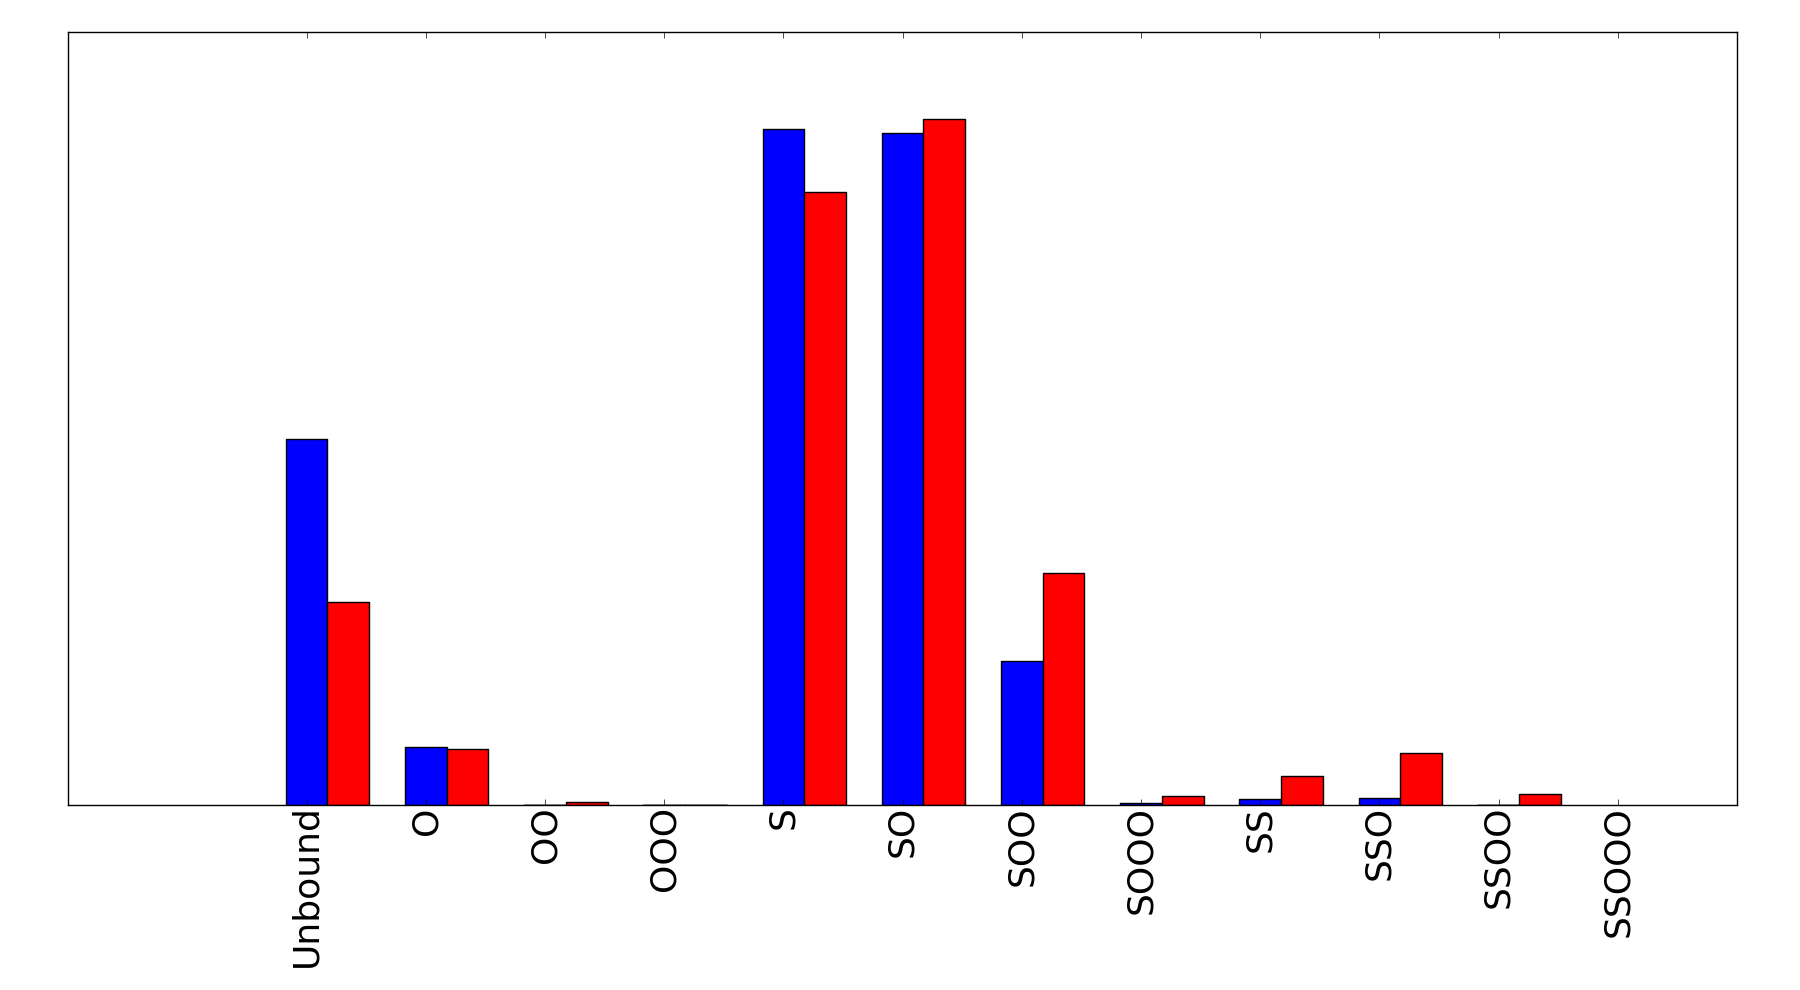
\includegraphics[scale=1.0]{images/coordination/so2-bonding-coordinations.png}
		\caption{Distribution of bonding coordinations of the surface \suldiox~molecule. Each set of bars represents the amount of time spent in the particular coordination type, including the unbound coordination. The results for the cold (blue) and hot (red) temperatures are shown together. At the high temperature the \suldiox~bonding becomes more complex with more bonds to the sulfur and oxygen atoms. The lower coordination states are more dominated in the cold temperature. The naming scheme is similar to that of a previous scheme for water coordinations,\cite{Buch2005} applied to the \suldiox~molecule.}
		\label{fig:so2-bonding-coordinations}
	\end{center}
\end{figure}


\begin{figure}[h!]
	\begin{center}
		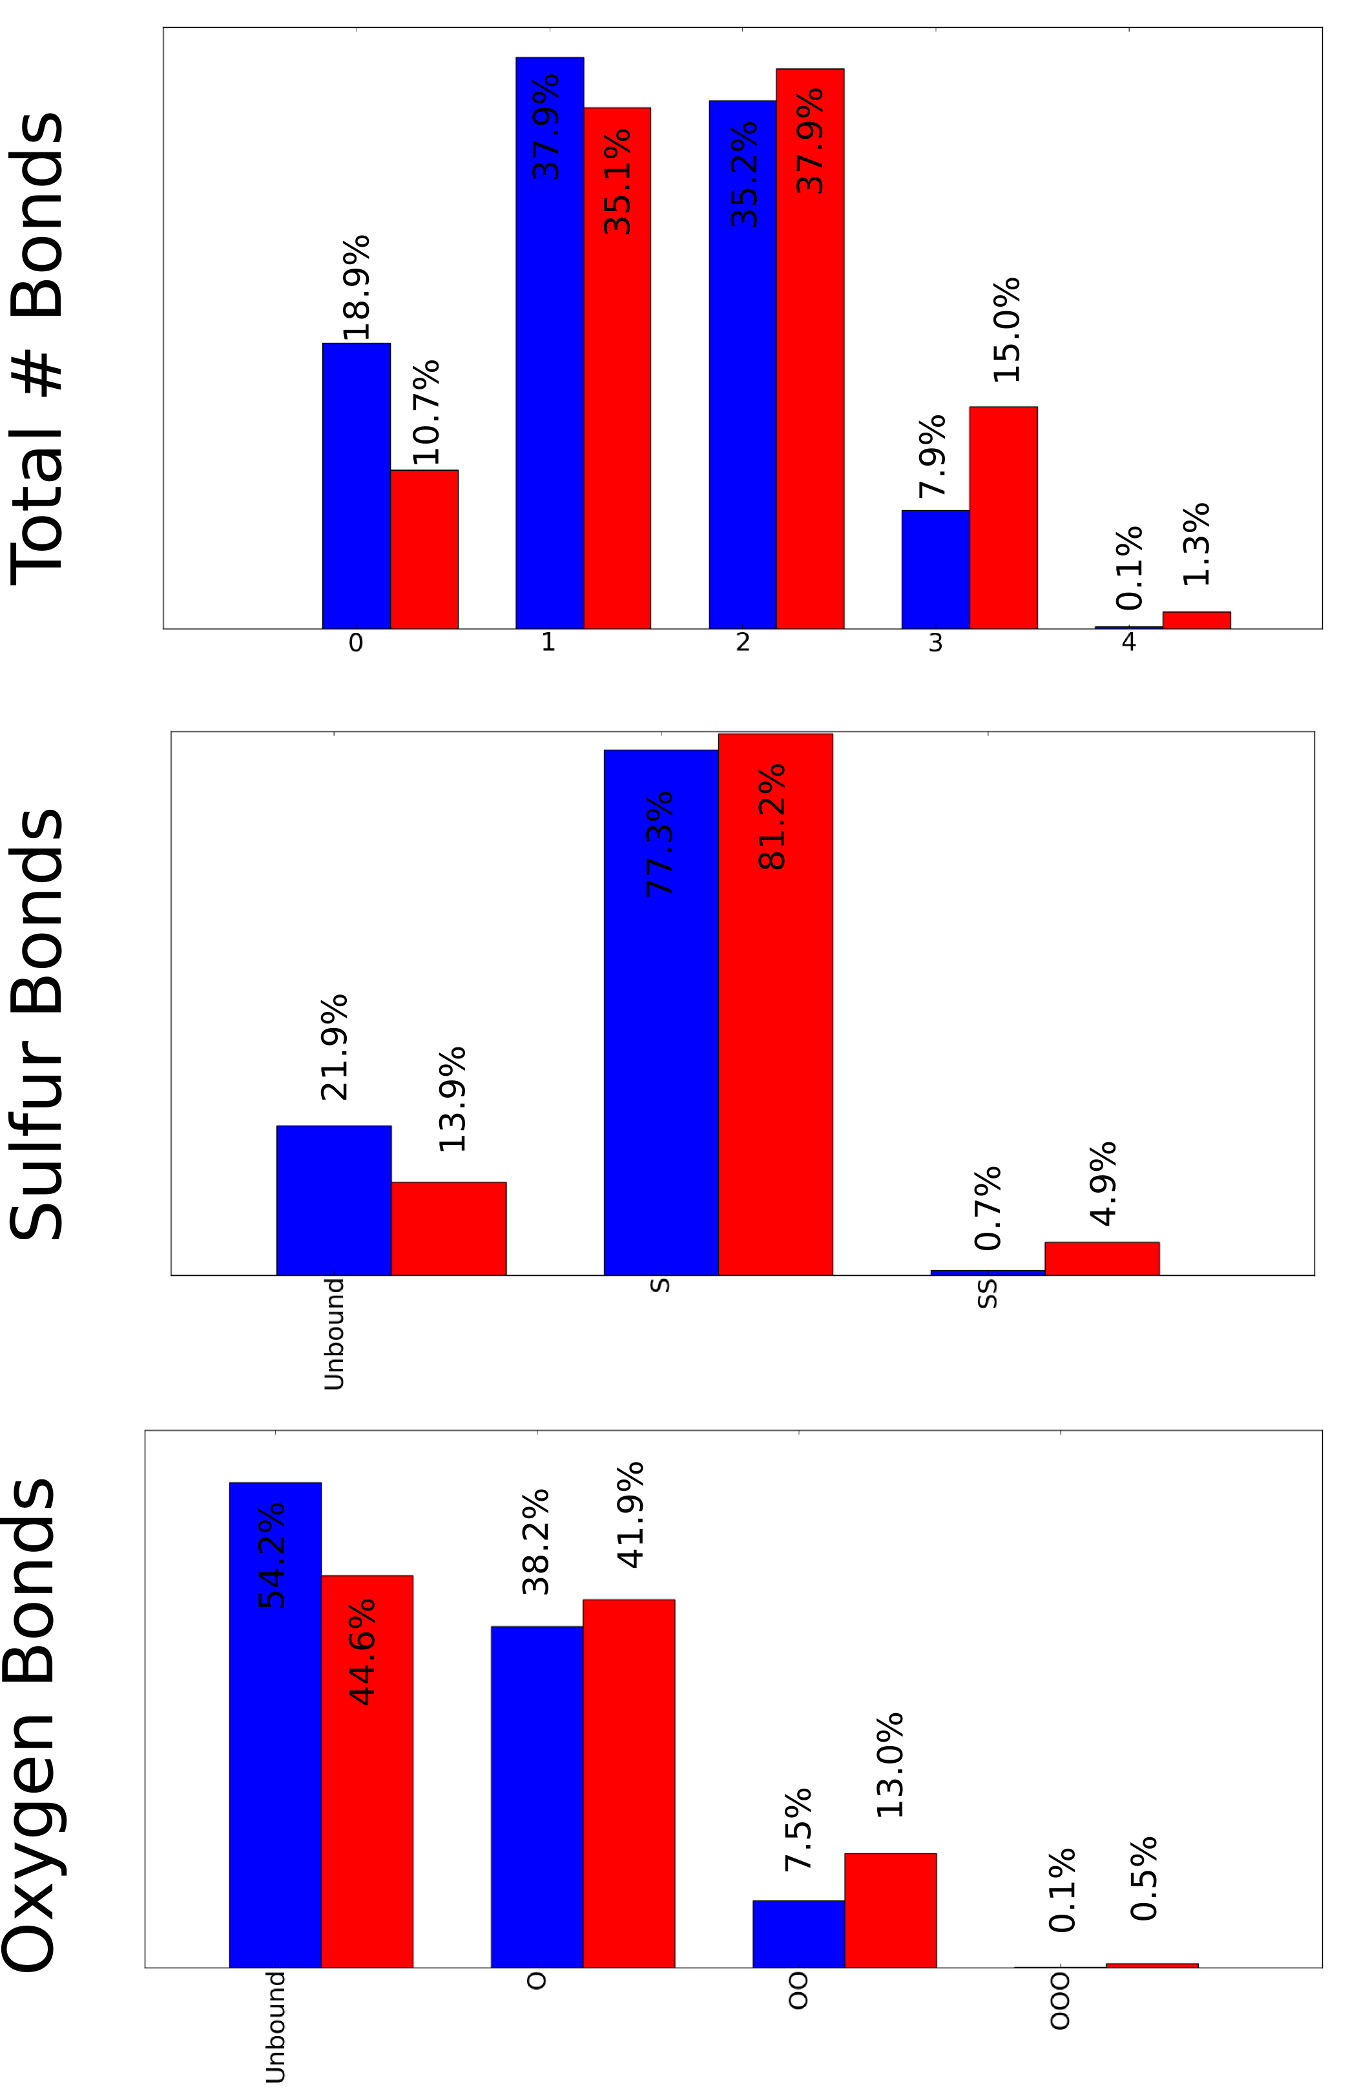
\includegraphics[scale=1.0]{images/coordination/coordination-breakdown.png}
		\caption{Bonding coordinations of the \suldiox~broken down into specific interactions. The total number of bonds to the molecule (top) are shown regardless of coordination type. The total number of bonds through either the sulfur atom (center) or through both of the oxygens (bottom). The \suldiox~primarily forms one or two bonds to the surface waters. The sulfur atom mostly bonds to a single water oxygen. Between the two \suldiox~oxygen atoms, the molecule mostly does not bond to the water hydrogens, or forms a single hydrogen-bond.}
		\label{fig:coordination-breakdown}
	\end{center}
\end{figure}

